\begin{frame}
  \begin{block}{How common are these clauses?}
    \begin{itemize}
    \item In the TPTP library (14k problems)
    \item 6000 different formulas that may result in positive
      equalities between variables
    \end{itemize}
  \end{block}
\end{frame}

\begin{frame}
  \begin{center}
    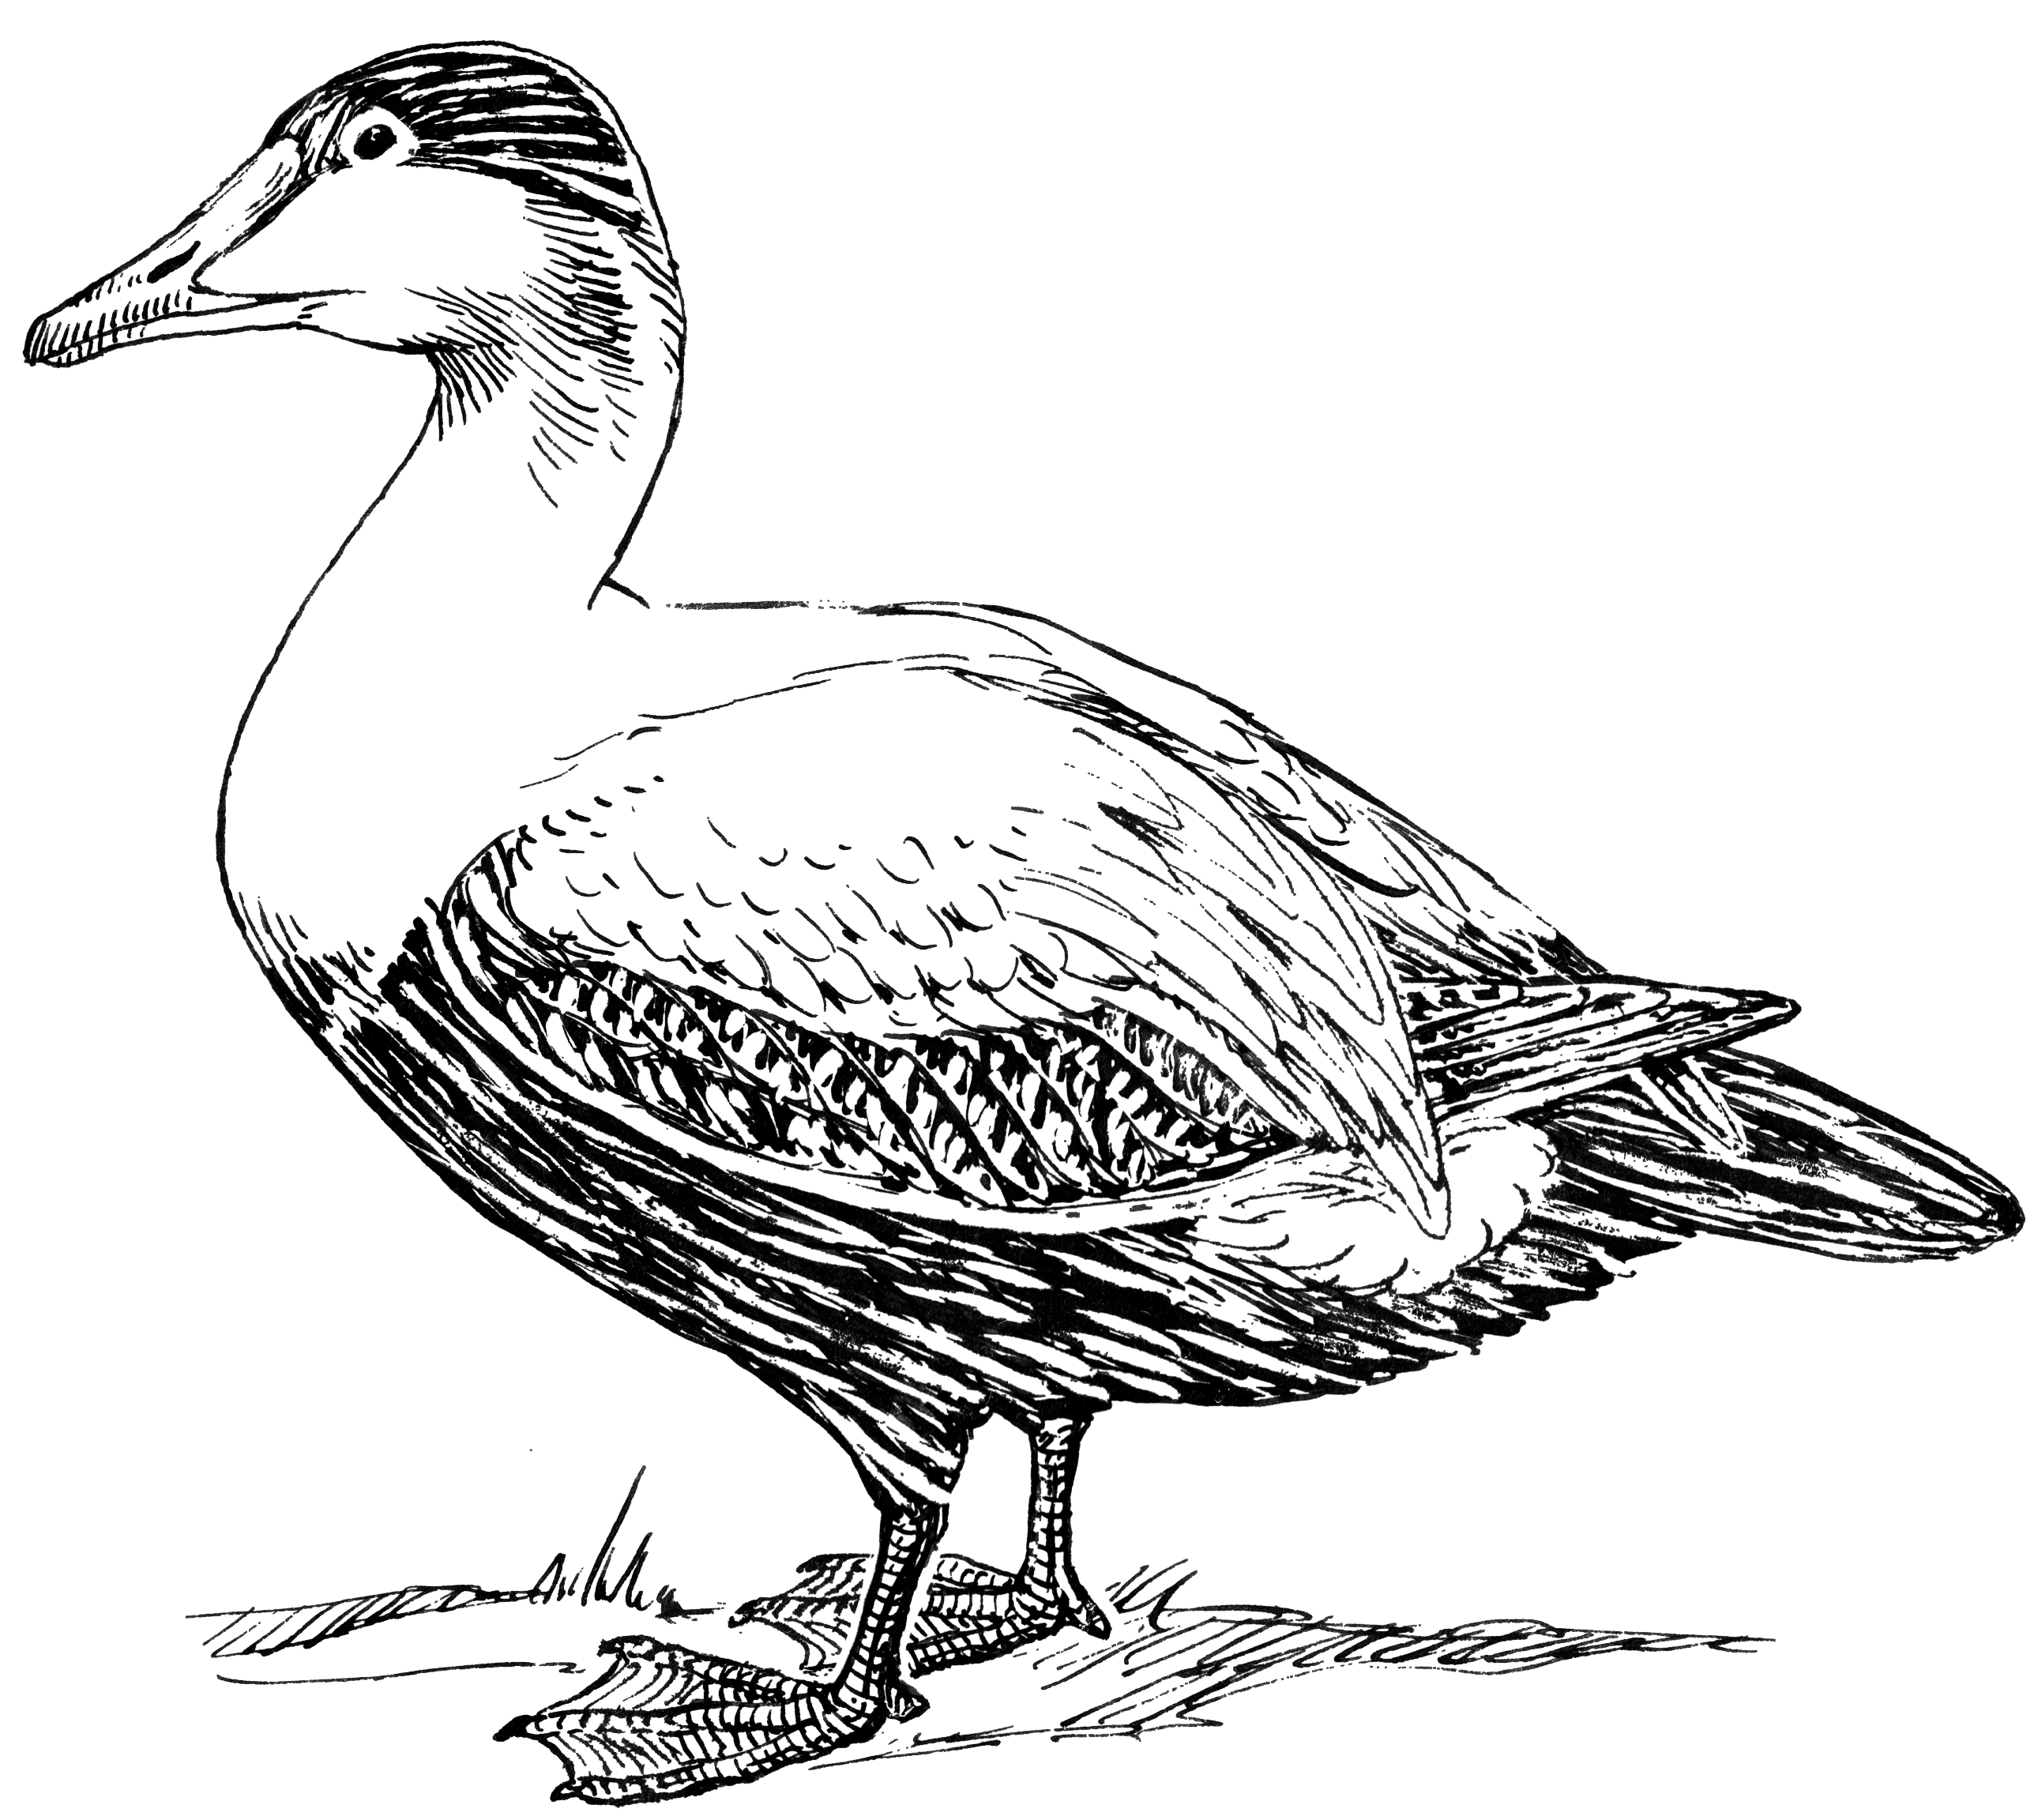
\includegraphics[width=.25\textwidth]{duck}
    
    \textit{If it looks like a duck and quacks like a duck\\ but it needs
    batteries,\\you probably have the wrong abstraction.}
  \end{center}
\end{frame}

\begin{frame}{Things that look like extensionality\dots}
  \begin{block}{Injectivity of constructors}
    \[
    succ(x) \neq succ(y) \lor x = y
    \]
    What happens if we treat this as an extensionality axiom?
  \end{block}
  
  \begin{block}{Solution}
    No clauses with a disequality of the same sort as $x = y$
  \end{block}
\end{frame}

\begin{frame}{Things that look like extensionality\dots}
  \begin{block}{Axiomatization of arrays}
    \[
    i = j \lor select(store(a,i,e), j) = select(a, j)
    \]
  \end{block}

  \begin{block}{Solution}
    No clauses with an equality other than the one among variables
  \end{block}
\end{frame}

\begin{frame}{Things that look like extensionality\dots}
  \begin{block}{Very long clauses}
    {\scriptsize
    \begin{gather*}
    x_4 = x_6 \lor ssSkC0 \lor \neg in(x_6 , x_7 ) \lor \neg front(x_7
    ) \lor \neg furniture(x_7 ) \lor \neg seat(x_7 ) \\ \lor \neg
    fellow (x_6 ) \lor \neg man(x_6 ) \lor \neg young(x_6 ) \lor \neg
    seat(x_5 ) \lor \neg furniture(x_5 ) \lor \neg front(x_5 ) \\ \lor
    \neg in(x_4 , x_5 ) \lor \neg young(x_4 ) \lor \neg man(x_4 ) \lor
    \neg fellow (x_4 ) \lor \neg in(x_2 , x_3 ) \lor \neg city(x_3 )
    \\ \lor \neg hollywood (x_3 ) \lor \neg event(x_2 ) \lor \neg
    barrel (x_2 , x_1 ) \lor \neg down(x_2 , x_0 ) \\ \lor \neg old
    (x_1 ) \lor \neg dirty(x_1 ) \lor \neg white(x_1 ) \lor \neg car
    (x_1 ) \lor \neg chevy(x_1 ) \\ \lor \neg street(x_0 ) \lor \neg
    way(x_0 ) \lor \neg lonely(x_0 )
    \end{gather*}
    }
  \end{block}

  \begin{block}{Solution}
    Limit the number of literals in extensionality clauses
  \end{block}
\end{frame}

\begin{frame}{Options to control ext\_rec}
  \begin{itemize}
  \item known: only applies to known set and array extensionality axioms
  \item all: applies the heuristics
  \end{itemize}
\end{frame}
